\documentclass{standalone}
\usepackage{tikz}
\usepackage{ctex,siunitx}
\setCJKmainfont{Noto Serif CJK SC}
\usepackage{tkz-euclide}
\usepackage{amsmath}
\usetikzlibrary{patterns, calc}
\usetikzlibrary {decorations.pathmorphing, decorations.pathreplacing, decorations.shapes,}

\begin{document}
\small
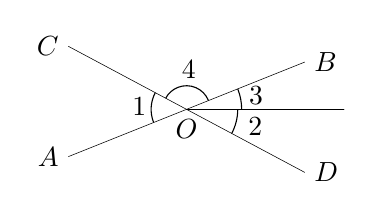
\begin{tikzpicture}[>=stealth,scale=1]
  \tkzSetUpPoint[fill=black]
  % \useasboundingbox(-1,-0.75)rectangle(3.7,1.4);
  \tkzDefPoints{-1.5/.4/A, -1.5/1.8/C, 0/1/O, 1.5/.2/D, 1.5/1.6/B, 2/1/E}
  \tkzDrawSegments(A,B C,D O,E)
  \tkzLabelPoints[left](A,C)
  \tkzLabelPoints[right](B,D)
  \tkzLabelPoints[below](O)
  \tkzMarkAngles[mark=none, size=.45](C,O,A)
  \tkzMarkAngles[mark=none, size=.65](D,O,E)
  \tkzMarkAngles[mark=none, size=.7](E,O,B)
  \tkzMarkAngles[mark=none, size=.3](B,O,C)
  \tkzLabelAngle[pos=.6](C,O,A){1}
  \tkzLabelAngle[pos=.9](D,O,E){2}
  \tkzLabelAngle[pos=.9](E,O,B){3}
  \tkzLabelAngle[pos=.5](B,O,C){4}
\end{tikzpicture}
\end{document}